\documentclass[../main.tex]{subfiles}
\begin{document}

\section{IoT Application (Traffic Light Calculator)}\label{sec:iot}

% Design Concepts
We implemented an IoT Application managing some crossing's traffic light, 
augmented with (mocked) self-driving car technology and image recognition. 
The road intersection contains various cameras and sensors. 
These allow for dynamically adapting light phases to current traffic, 
weather conditions, and intentions of road users. 

\subsection{Application Design}\label{ssec:iotApplicationStructure}

We simplified this conplex scenario by only representing a single city traffic light 
that shows German standard light phases: 
The traffic light gets yellow (for a few seconds) then red if there are no cars attempting to cross 
or if there is a car that approaches dangerously fast (and thus has to be stopped). 
It switches to green (via yellow-red) otherwise. 

For dangerous road conditions (like bad weather), each light switch is delayed. 
In the special case that an emergency (ambulance/police) is detected, 
the light instantly switches to yellow and blink 
in order to warn all participants. 
We assume cars only cross on green and pedestrians only cross on red.

Detailed descriptions of how the application is structured 
and of each function's purpose are depicted in 
\Cref{fig:iotArchitectureDiagram} and \Cref{tab:iotFunctionOverview}.
Databases are needed for aggregating/coordinating multiple functions' states
and for storing traffic statistics. 

\begin{figure}
\begin{center}
  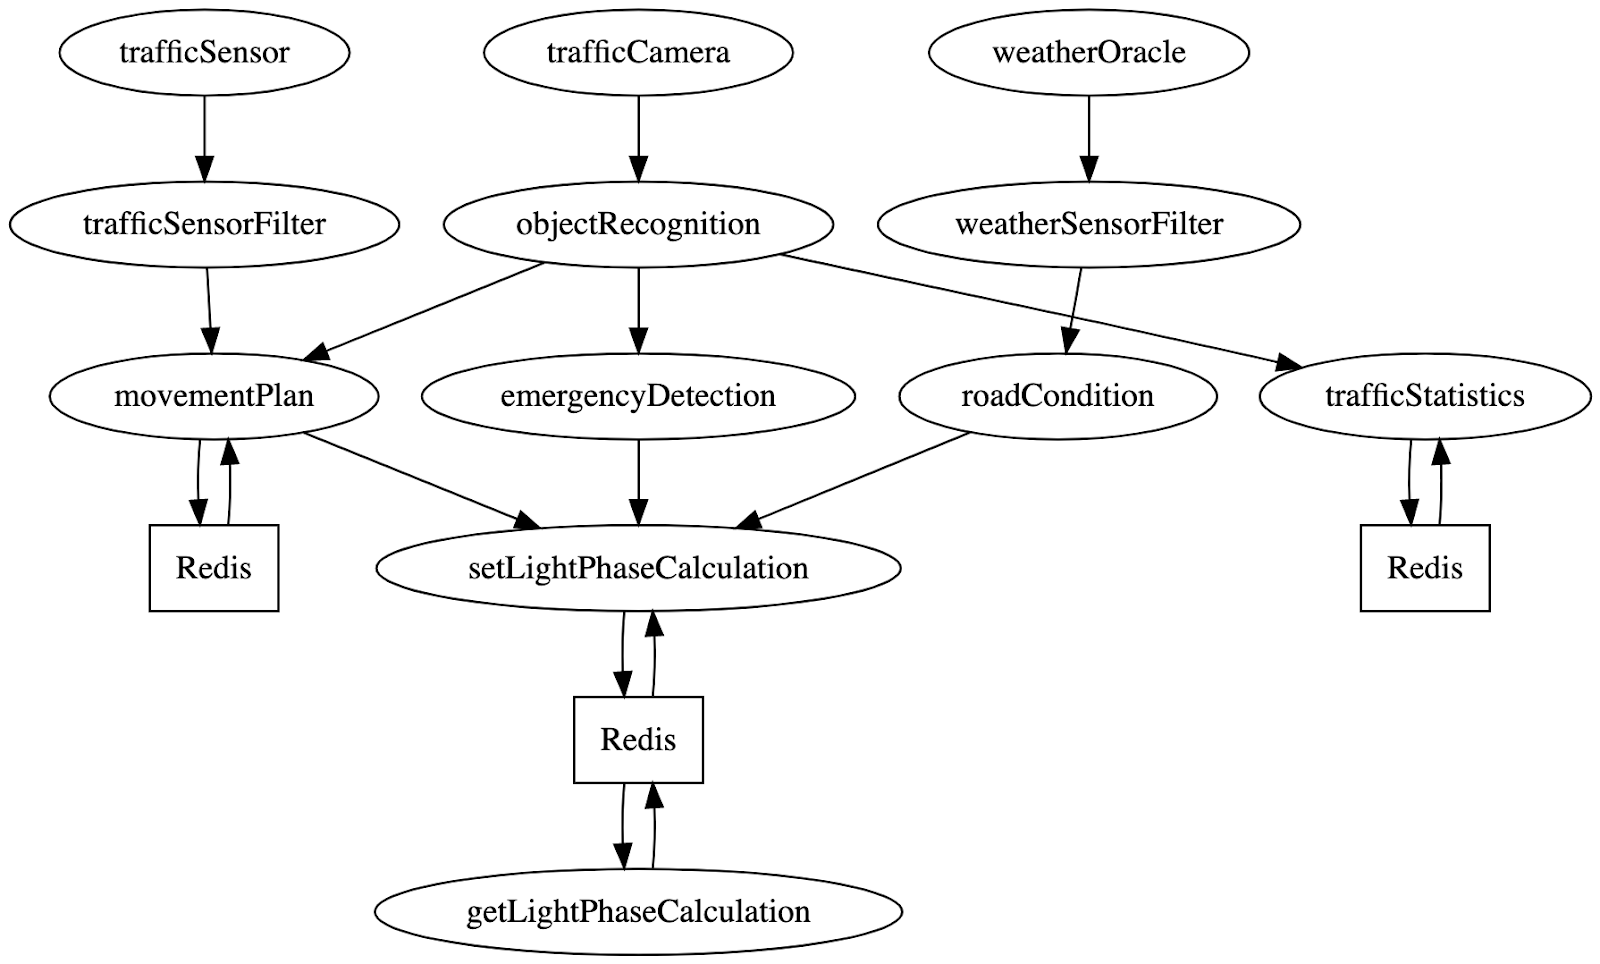
\includegraphics[width=\linewidth,keepaspectratio]{./iot-architecture-diagram.png}
\end{center}
\caption[IoT Architecture Diagram]{%
  Architecture diagram of our traffic light application.
  All functions communicate internally with each other via our library's RPC system
  and are thus automatically measured at runtime.
  The IoT devices in the top row (i.e.\@ trafficSensor, trafficCamera and weatherOracle) 
  represent the experiment's workload and are thus mocked in our setup (e.g.\@ by artillery workloads).%
}%
\label{fig:iotArchitectureDiagram}
\end{figure}

\begin{longtable}{l l} 
  \caption[IoT Function Overview]{IoT Function Overview\vspace*{1mm}}\label{tab:iotFunctionOverview}\\
  \textbf{Function} & \multicolumn{1}{c}{\textbf{Description}}\\ 
  \toprule
  %\endhead{}%
  trafficsensorfilter & \makecell[{{p{11cm}}}]{Filters incoming traffic sensor data (e.g.\@ car speeds and directions),
    removing erroneous inputs.}\\
  \midrule[0.02em]
  objectrecognition & \makecell[{{p{11cm}}}]{Analyses an uploaded camera image and detects different vehicles.}\\
  \midrule[0.02em]
  weathersensorfilter & \makecell[{{p{11cm}}}]{Filters incoming weather sensor data, removing erroneous inputs.}\\
  \midrule[0.02em]
  movementplan & \makecell[{{p{11cm}}}]{Uses database to aggregate found objects with their traffic attributes. 
    Submits to setlightphasecalculation.}\\
  \midrule[0.02em]
  emergencydetection & \makecell[{{p{11cm}}}]{Sends emergency status to setlightphasecalculation if respective 
    objects were detected.}\\
  \midrule[0.02em]
  roadcondition & \makecell[{{p{11cm}}}]{Evaluates (and scores) current road condition according to 
    incoming weather data. Submits to setlightphasecalculation.}\\
  \midrule[0.02em]
  trafficstatistics & \makecell[{{p{11cm}}}]{Saves seen objects to database for potential future analysis.}\\
  \midrule[0.02em]
  setlightphasecalculation & \makecell[{{p{11cm}}}]{Aggragates all received input in database. 
    Perpetually calculates light phases and updates traffic light in database. 
    Responds to emergencies immediately (i.e.\@ without wait).}\\
  \midrule[0.02em]
  getlightphasecalculation & \makecell[{{p{11cm}}}]{Returns current light phase.}\\
  \midrule[0.02em]
  \bottomrule
\end{longtable}

Exact Function I/O specification can also be looked up within the source code\footnotemark.
There, each function has its I/O behaviour (including individual examples) documented.
\footnotetext{\url{https://github.com/FaaSterMetrics/experiments/tree/master/experiments/iot/functions}}

\subsection{Benchmarking Properties}\label{ssec:iotApplicationProperties}

In comparison to the webshop application, the IoT traffic light calculator combines data from multiple input sources
which are heterogeneous both in their structural and their frequency behaviour. 
In order to do so, the application heavily relies on the external database.

Those inputs also vary from continuous image and sensor streams to signals by incoming vehicles. 
Additionally, the introduced operations require combination of multiple data sources, 
as well as passing information to multiple subsequent operations, 
leading to a branched pipeline structure (\Cref{fig:iotArchitectureDiagram}). %TODO formulation?
While some functions only perform bookkeeping functions, others such as the emergency detection have strict latency requirements.

Regarding the technical side of IoT infrastructure most major platforms nowadays include tailored stacks for IoT deployments\footnotemark.
Those offer managed device management/data acquisition stack (MQTT, trigger systems)
and integration into their broader cloud platform services including FaaS.
We consider our scope to be only the FaaS system's reaction to incoming IoT data. 
Therefore MQTT and trigger systems are neither tested nor built into our implementation. 
Only the FaaS functions themselves and database connections for storing or collecting information are needed.

\footnotetext{See e.g.\@ Azure IoT Edge (\url{https://docs.microsoft.com/en-us/azure/iot-edge}),
Google Cloud IoT (\url{https://cloud.google.com/solutions/iot}) and
AWS IoT Greengrass (\url{https://aws.amazon.com/iot/solutions/iot-edge})
}

\subsection{Specific Workloads}\label{ssec:iotSpecificWorkloads}

To complete the experiment, we also pre-defined some workload profiles which were automatized with \texttt{artillery}
(see \Cref{sec:sec:WorkloadsStructure}).
Naturally, each of those profiles leads to an individual experiment.
Thus, you should use the application's workload profile that reflects the situation you want to analyse the closest,
or develop your own one if required.
That said, the first described workload profile suits an average webshop scenario best and is therefore generally recommended.

\subsubsection{``Shibuya Crossing''}%
\label{ssub:iotShibuya}

This workload profile aims to simulate a modern city crossing with a large amount of actors,
hence the name `Shibuya Crossing'.
The most important part, however, is reflected in its temporal features:
The workload features a high amount of normal traffic for 5 minutes,
then being suddenly interrupted by a single emergency.
Of course, following the declared goal of this application, this one emergency still has to change the traffic lights immediately.
Thus, we test if the deployed application can still react properly fast, 
if it has been stressed for a longer time period beforehand (most notably including its database).

The profile can be found in the repository's iot directory as 
\begin{tcolorbox}
\quad\texttt{workload-single-incident.yml}
\end{tcolorbox}

\subsubsection{``Breaking Dawn''}%
\label{ssub:iotDawn}

This workload profile basically features pure database and function pipeline testing, there are no triggered emergencies.
The general load increases gradually, thus representing regular city traffic in the morning.
Testing also lasts for five minutes by default.

The profile can be found in the repository's iot directory as 
\begin{tcolorbox}
\quad\texttt{workload-increasing-no-incidents.yml}
\end{tcolorbox}

\subsubsection{``Pampa-Ampel''}%
\label{ssub:iotPampaAmpel}

This workload profile contains a relatively low load, but regularly calls all functions the application has to offer,
for a total of 30 minutes.
Emergencies are triggered every 2 minutes and last 5 seconds each, 
thus periodically interrupting the usual light switching process.

The profile's name, ``Pampa-Ampel'' is German and jokingly references to the boredom of life in the countryside.
The profile can be found in the repository's iot directory as 
\begin{tcolorbox}
\quad\texttt{workload-low-load-regular-incidents.yml}
\end{tcolorbox}


\end{document}
